\chapter{Results, Conclusion and Future Work}

%Replace \lipsum with text.
% You may have as many sections as you please. This is just for reference.


In this chapter we will discuss the results of the VLAN application in terms of bandwidth for all the four different cases. We have also shown the results for the load balancing application. Finally we will conclude the results of both the applications and suggest future work which can be done to further extend the application into a full fledged SDN based solution for Baadal.

\section{Comparison of SDN based solution in terms of Bandwidth}

Figure \ref{fig:SamehostSameVLan} shows the comparison of bandwidth between two virtual machines belonging to same host and same VLan. It shows that the bandwidth attained for different sizes of packets is almost same for both the traditional and SDN based solution

\begin{figure}
\caption{Bandwidth comparison of traditional and SDN metworking in Same host Same VLan}
\centering
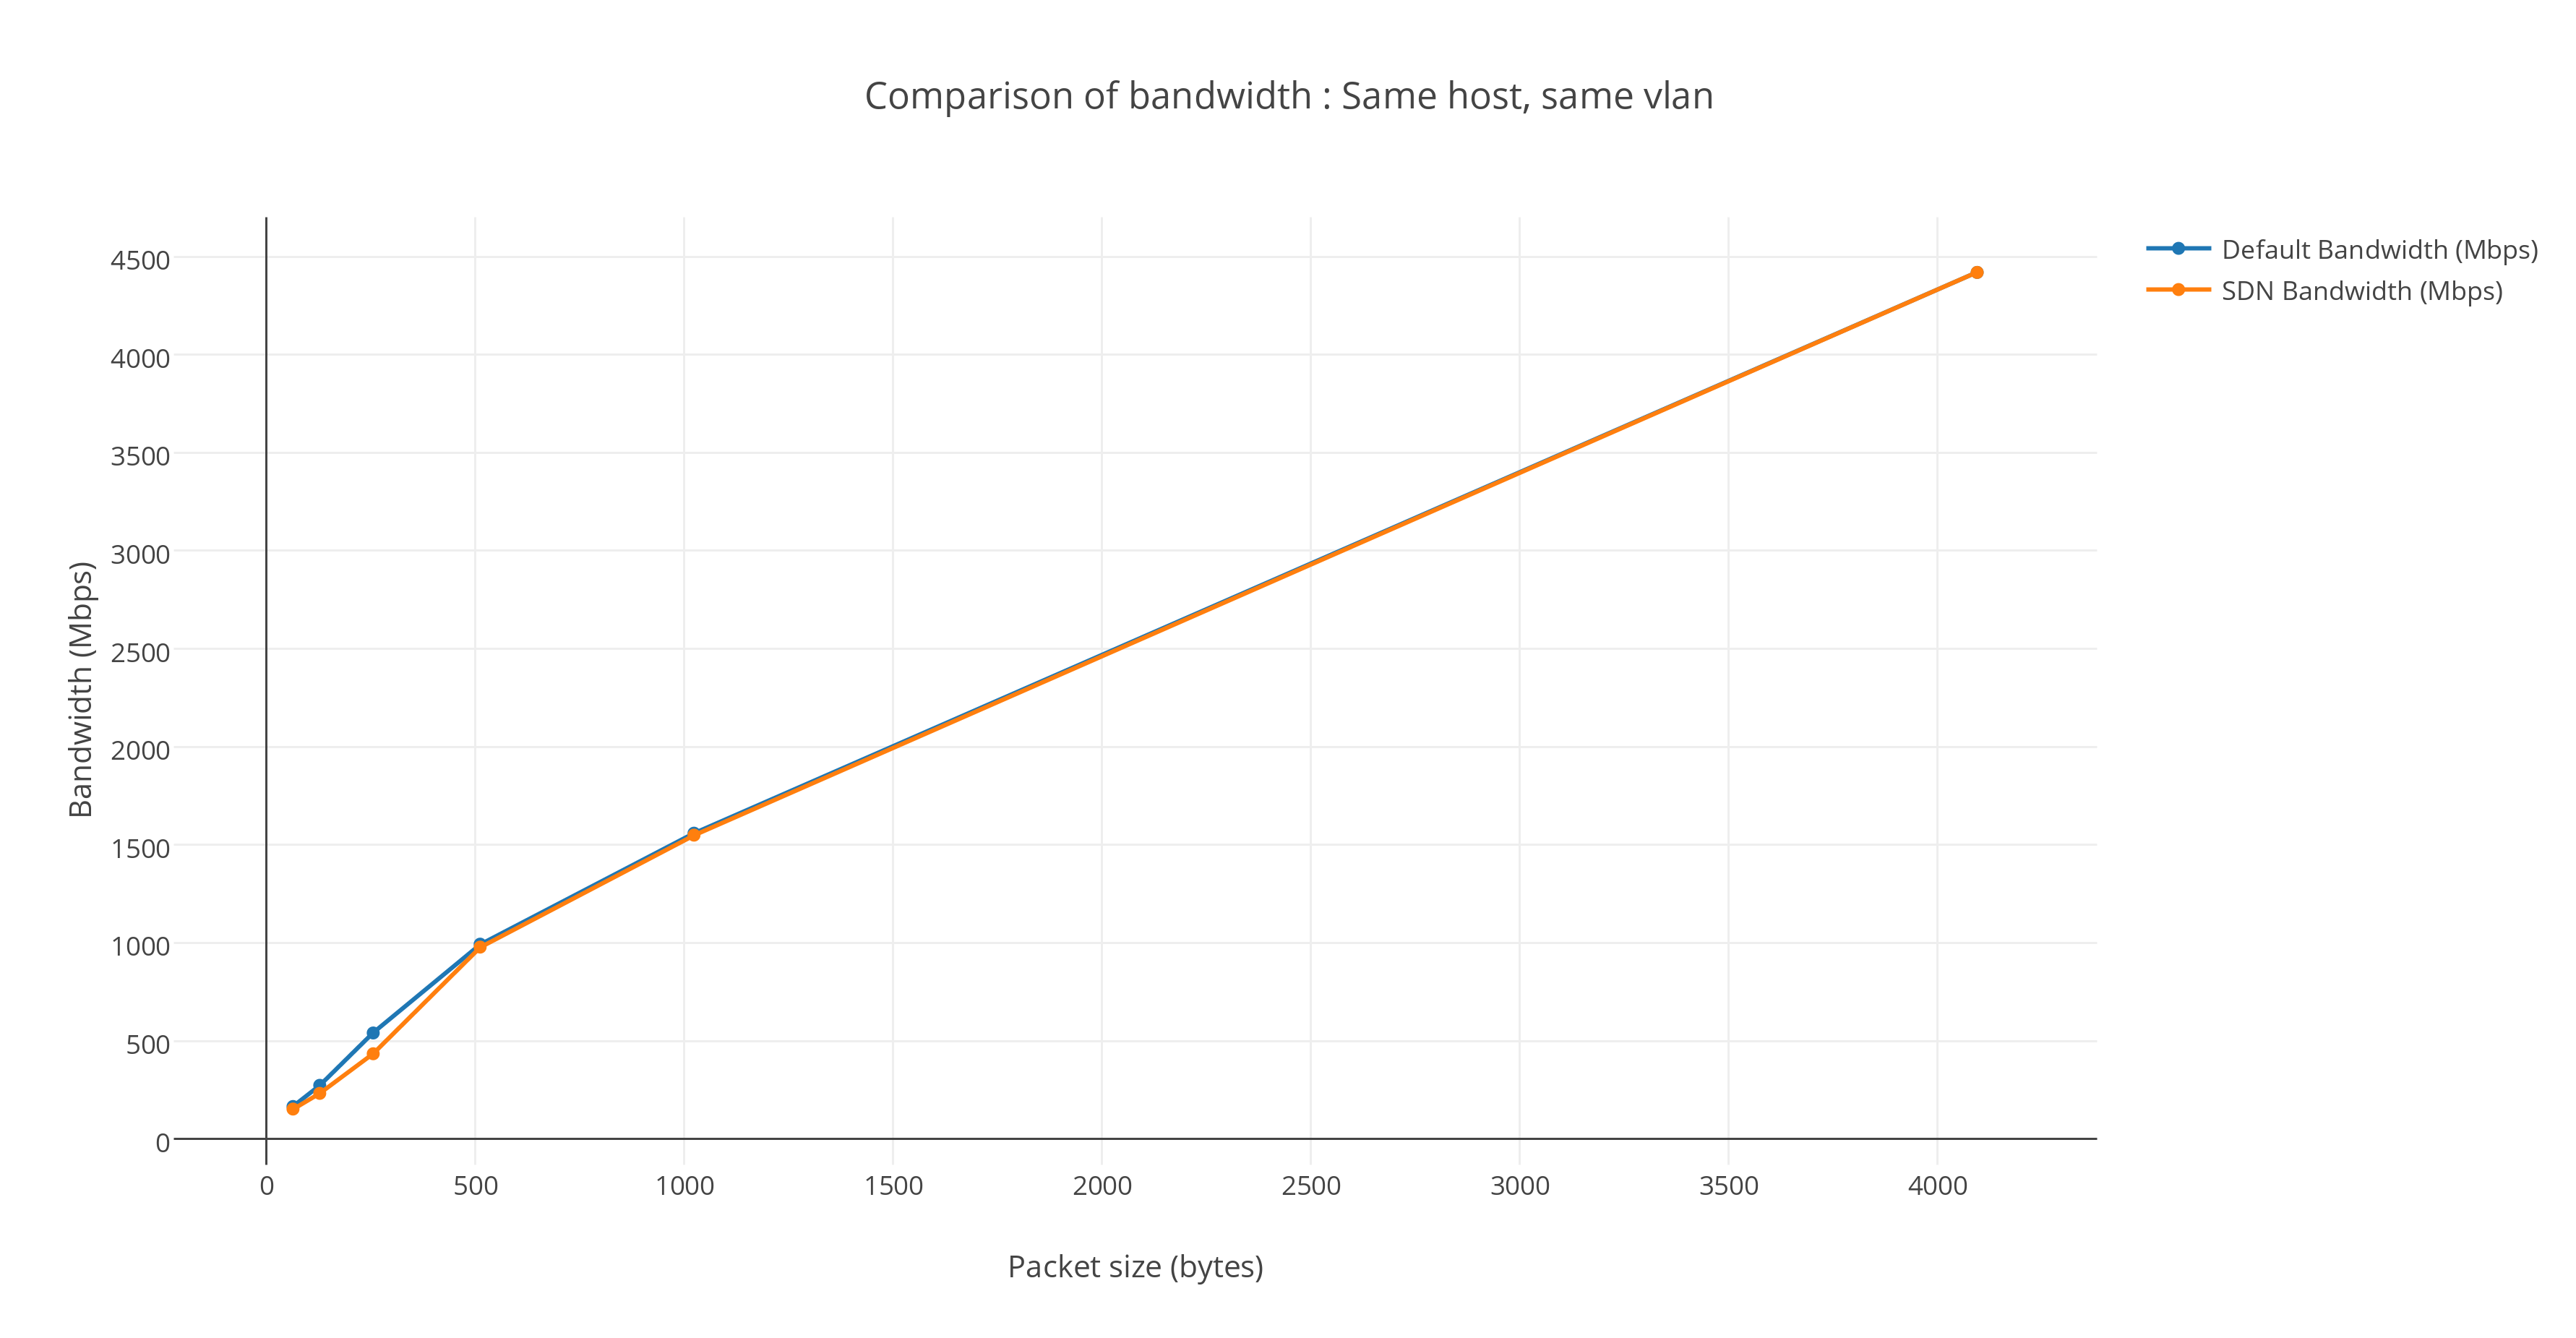
\includegraphics[width=11cm, height=5.5cm]{same_host_same_vlan}
\label{fig:SamehostSameVLan}
\end{figure}

\newpage
Figure \ref{fig:difhostsameVLan} shows the bandwidth comparison for VMs belonging to different host and same vlan. We can see that the bandwidth for different packet sizes achieved is much higher in case of SDN even though uniformity is less in traditional networking.
\begin{figure}
\caption{Bandwidth comparison of traditional and SDN metworking in Different host Same VLan}
\centering
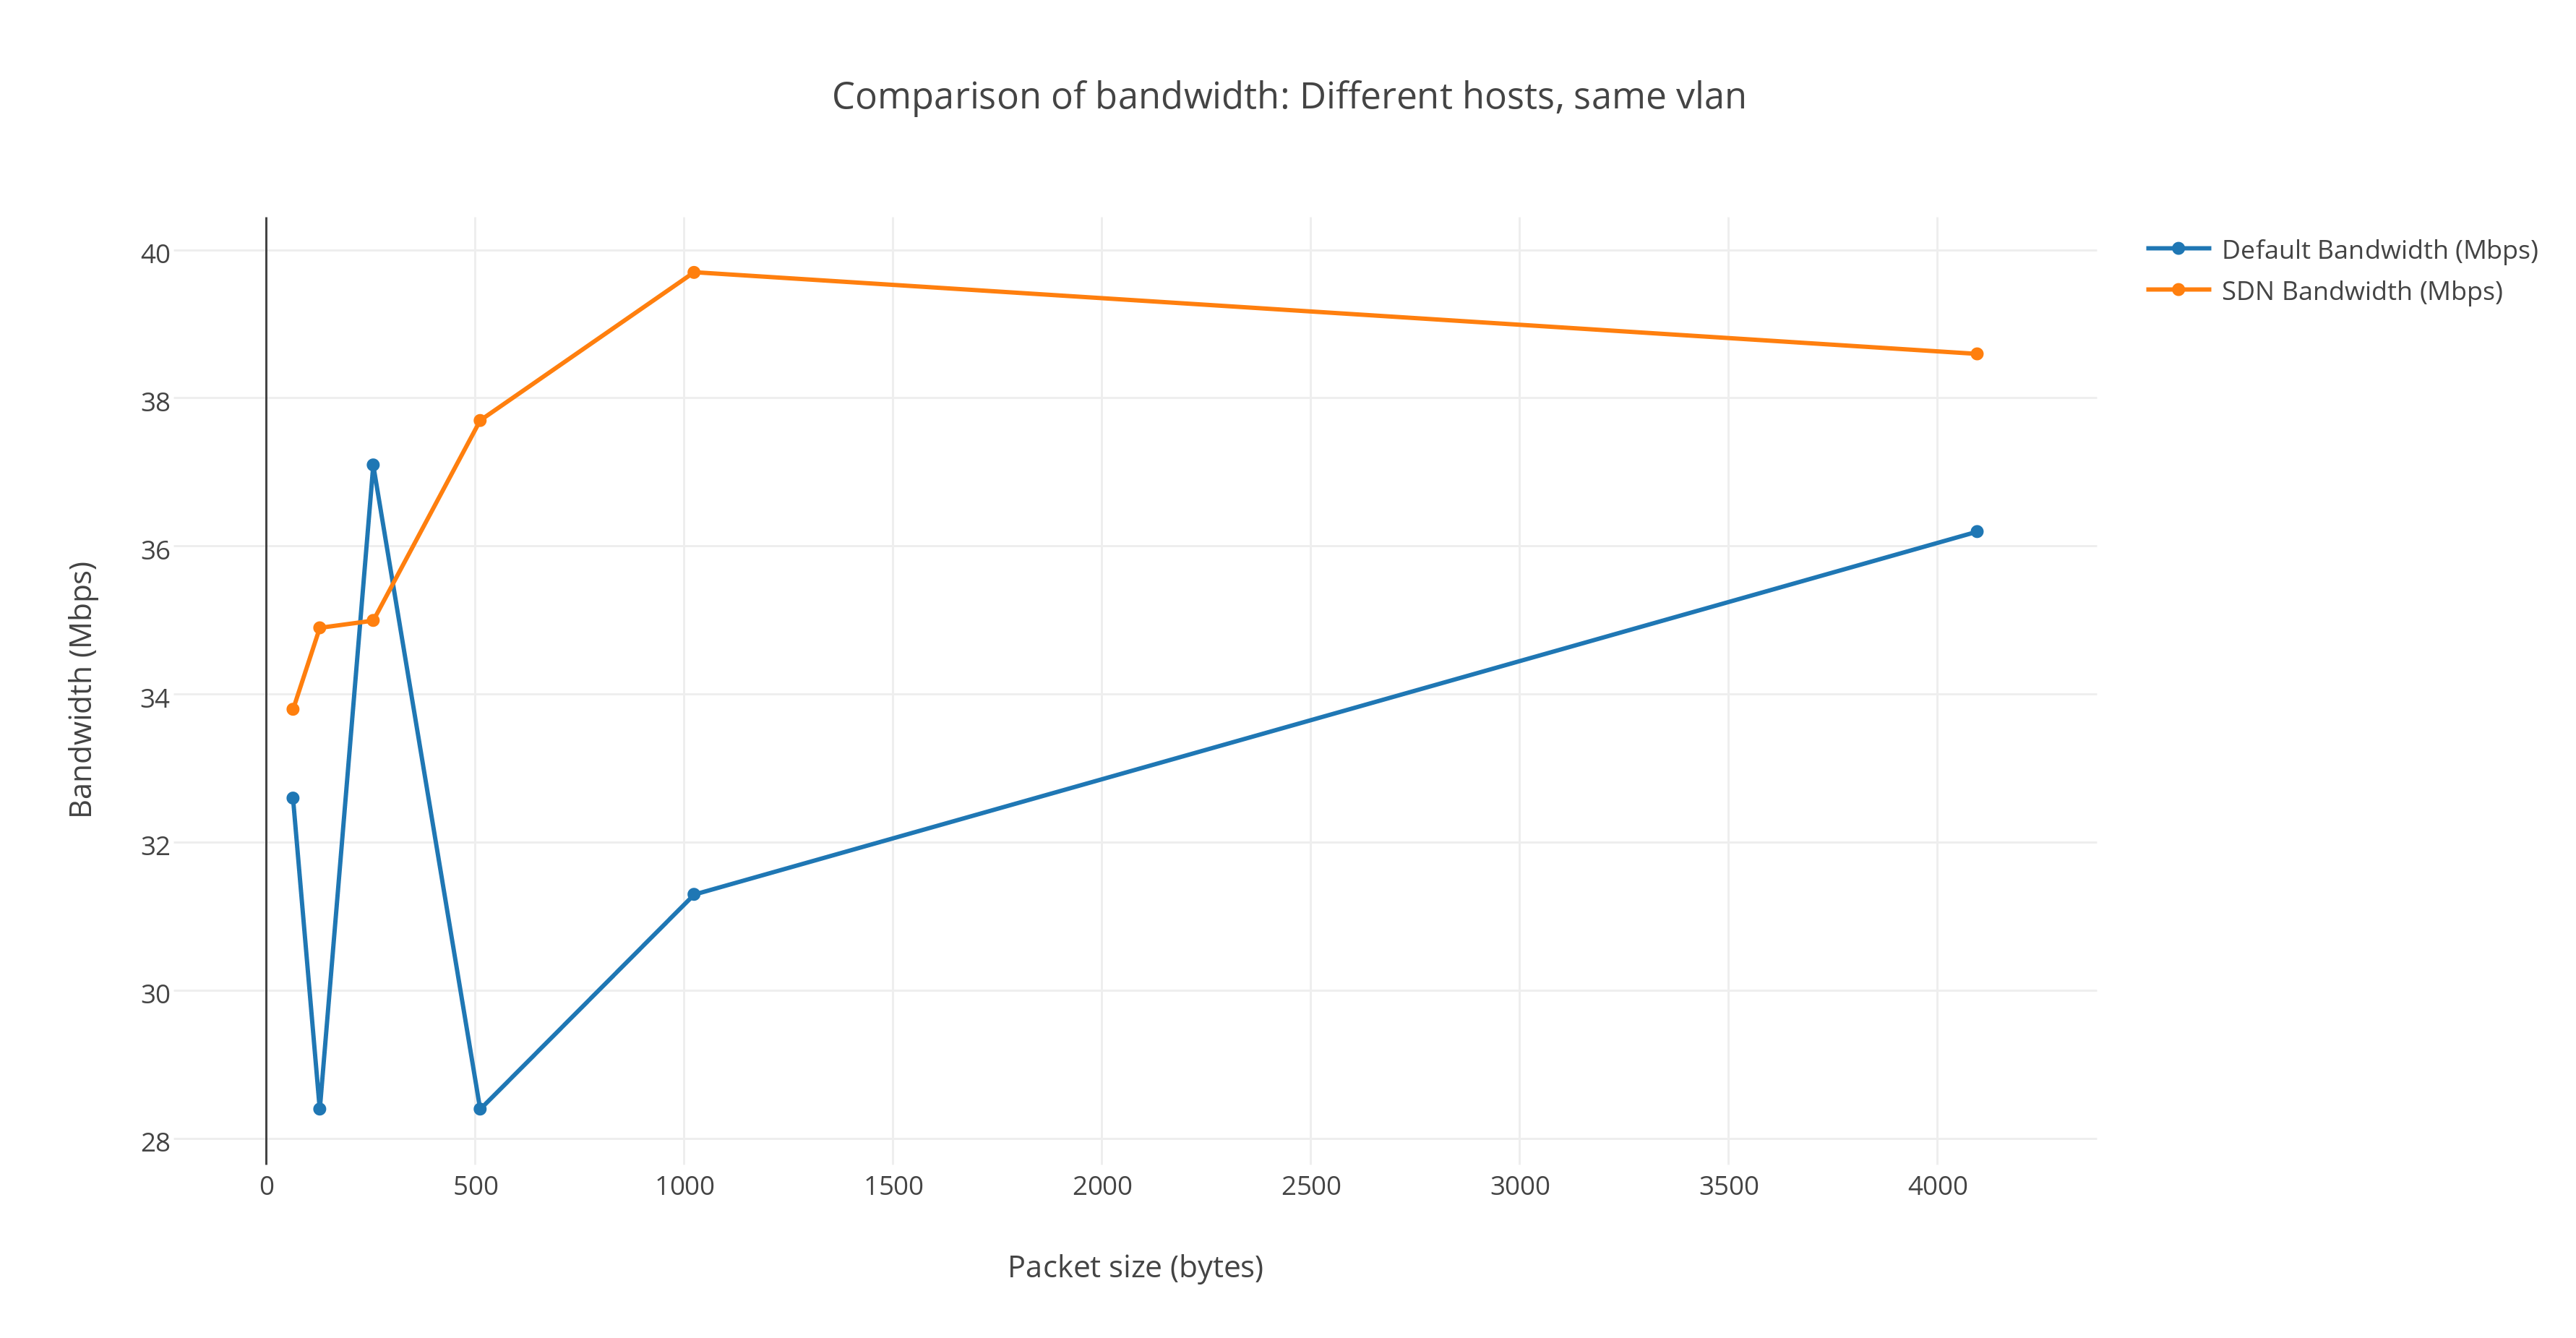
\includegraphics[width=11cm, height=7cm]{different_host_same_vlan}
\label{fig:difhostsameVLan}
\end{figure}

\newpage

The next case of comparison is for the VMs belonging to same host and different vlan. The plot \ref{fig:SamehostdifVLan} shows a huge improvement in bandwidth achieved with SDN solution. It is observed that with increasing packet size the SDN bandwidth increases while the traditional networking bandwidth almost remains same.

\begin{figure}
\caption{Bandwidth comparison of traditional and SDN networking in Same host Different VLan}
\centering
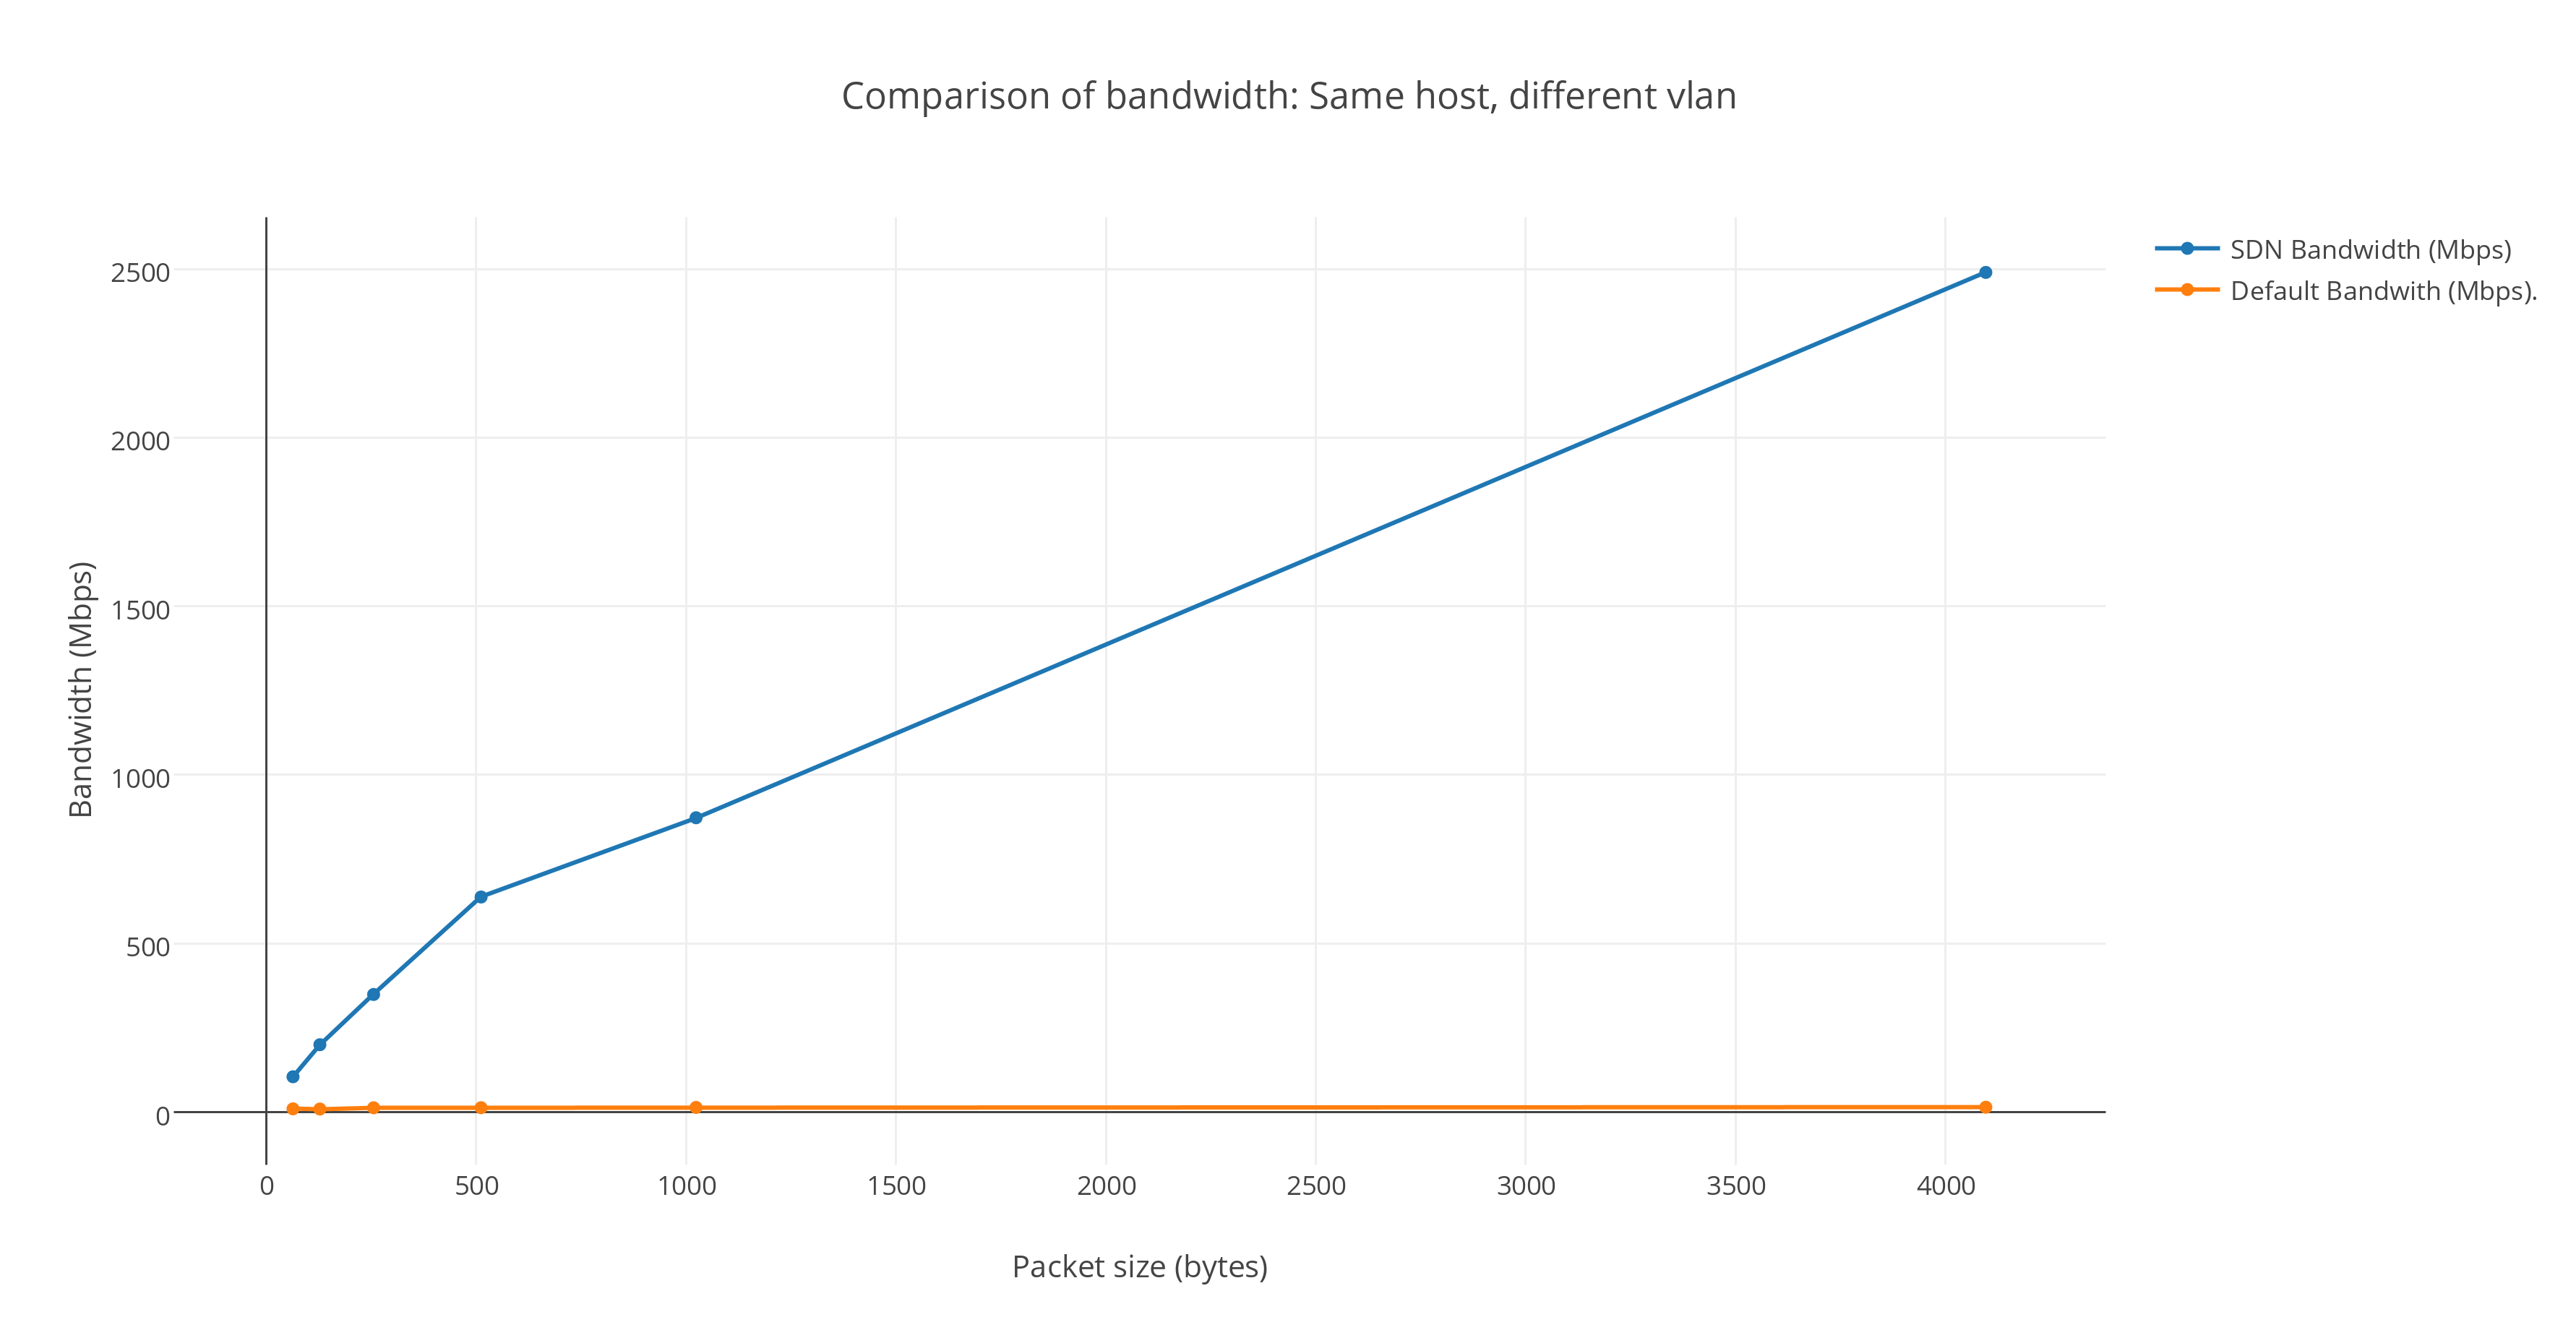
\includegraphics[width=1.0\textwidth]{same_host_different_vlan}
\label{fig:SamehostdifVLan}
\end{figure}

\newpage

The last case for the comparison is between VMs belonging to different hosts and different vlan. From the plot \ref{fig:difhostdifVLan} it can be observed that the difference in the bandwidth between SDN based solution and traditional networking  is higher for the smaller packet size unlike previous case. 

\begin{figure}[h]
\caption{Bandwidth comparison of traditional and SDN metworking in Different host Different VLan}
\centering
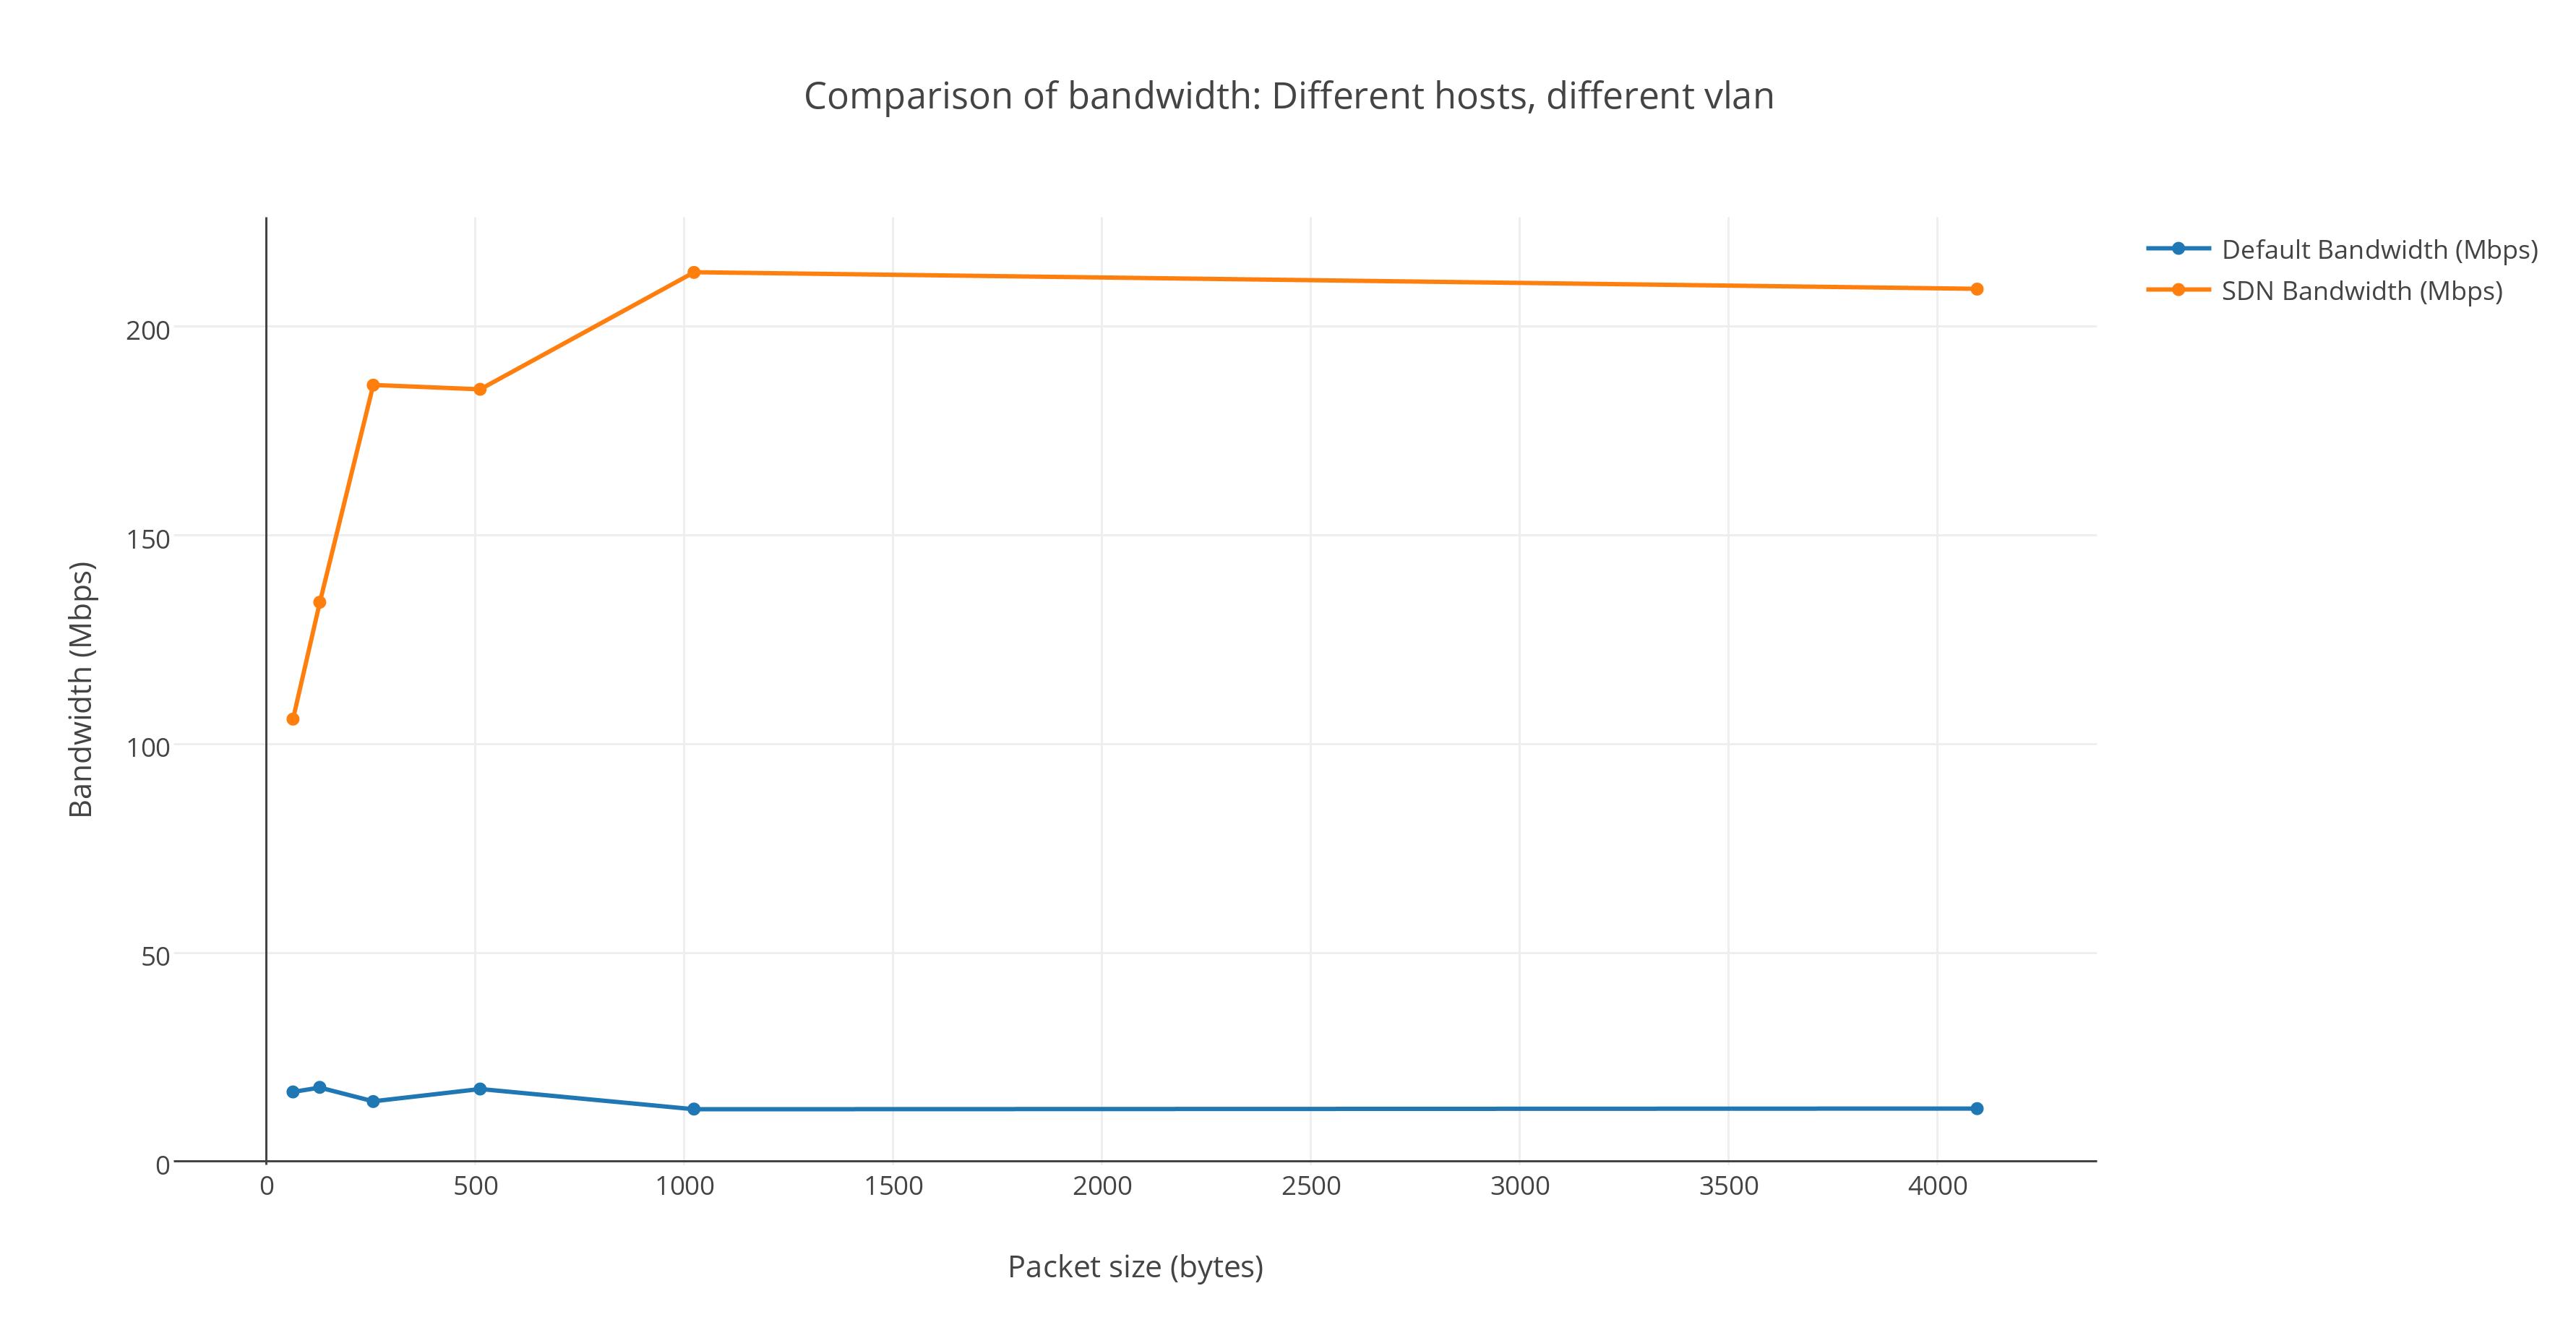
\includegraphics[width=1.0\textwidth]{different_host_different_vlan}
\label{fig:difhostdifVLan}
\end{figure}


\section{Results for VMs consolidation application}
\begin{figure}[h]
\caption{Heatmap showing network traffic between virtual machines}
\centering
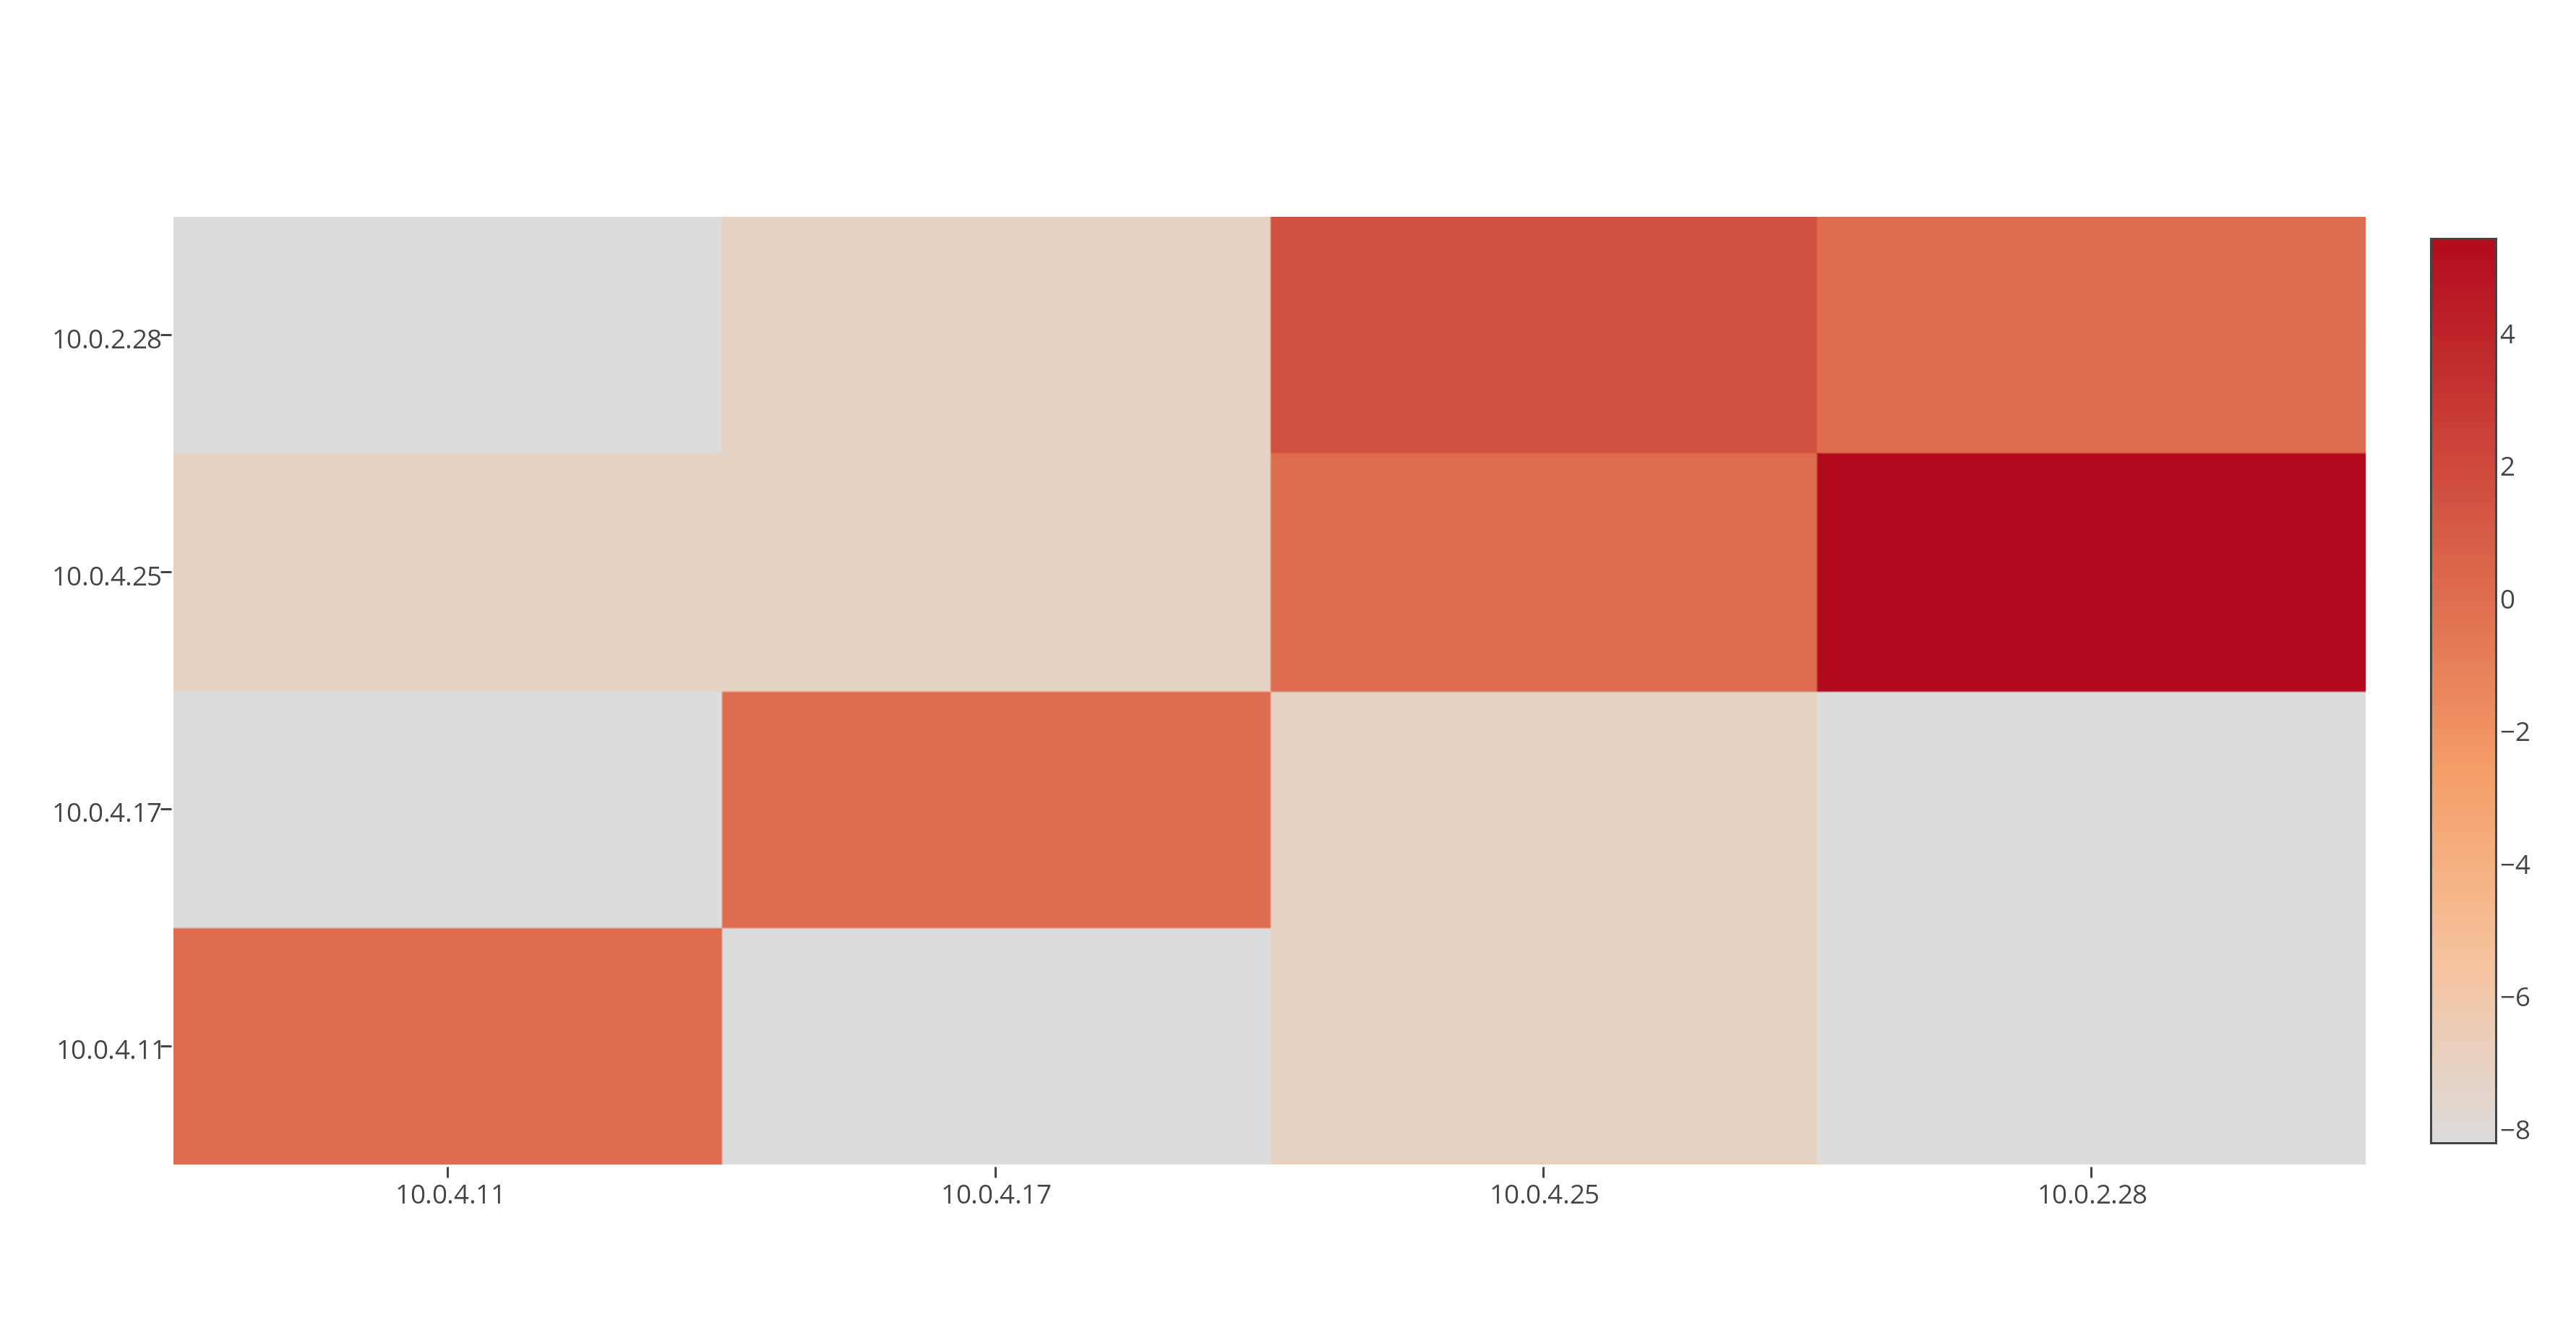
\includegraphics[width=0.9\textwidth]{vm_heatmap}
\end{figure}

\begin{figure}[h]
\caption{Heatmap showing network traffic between different hosts before VM migration}
\centering
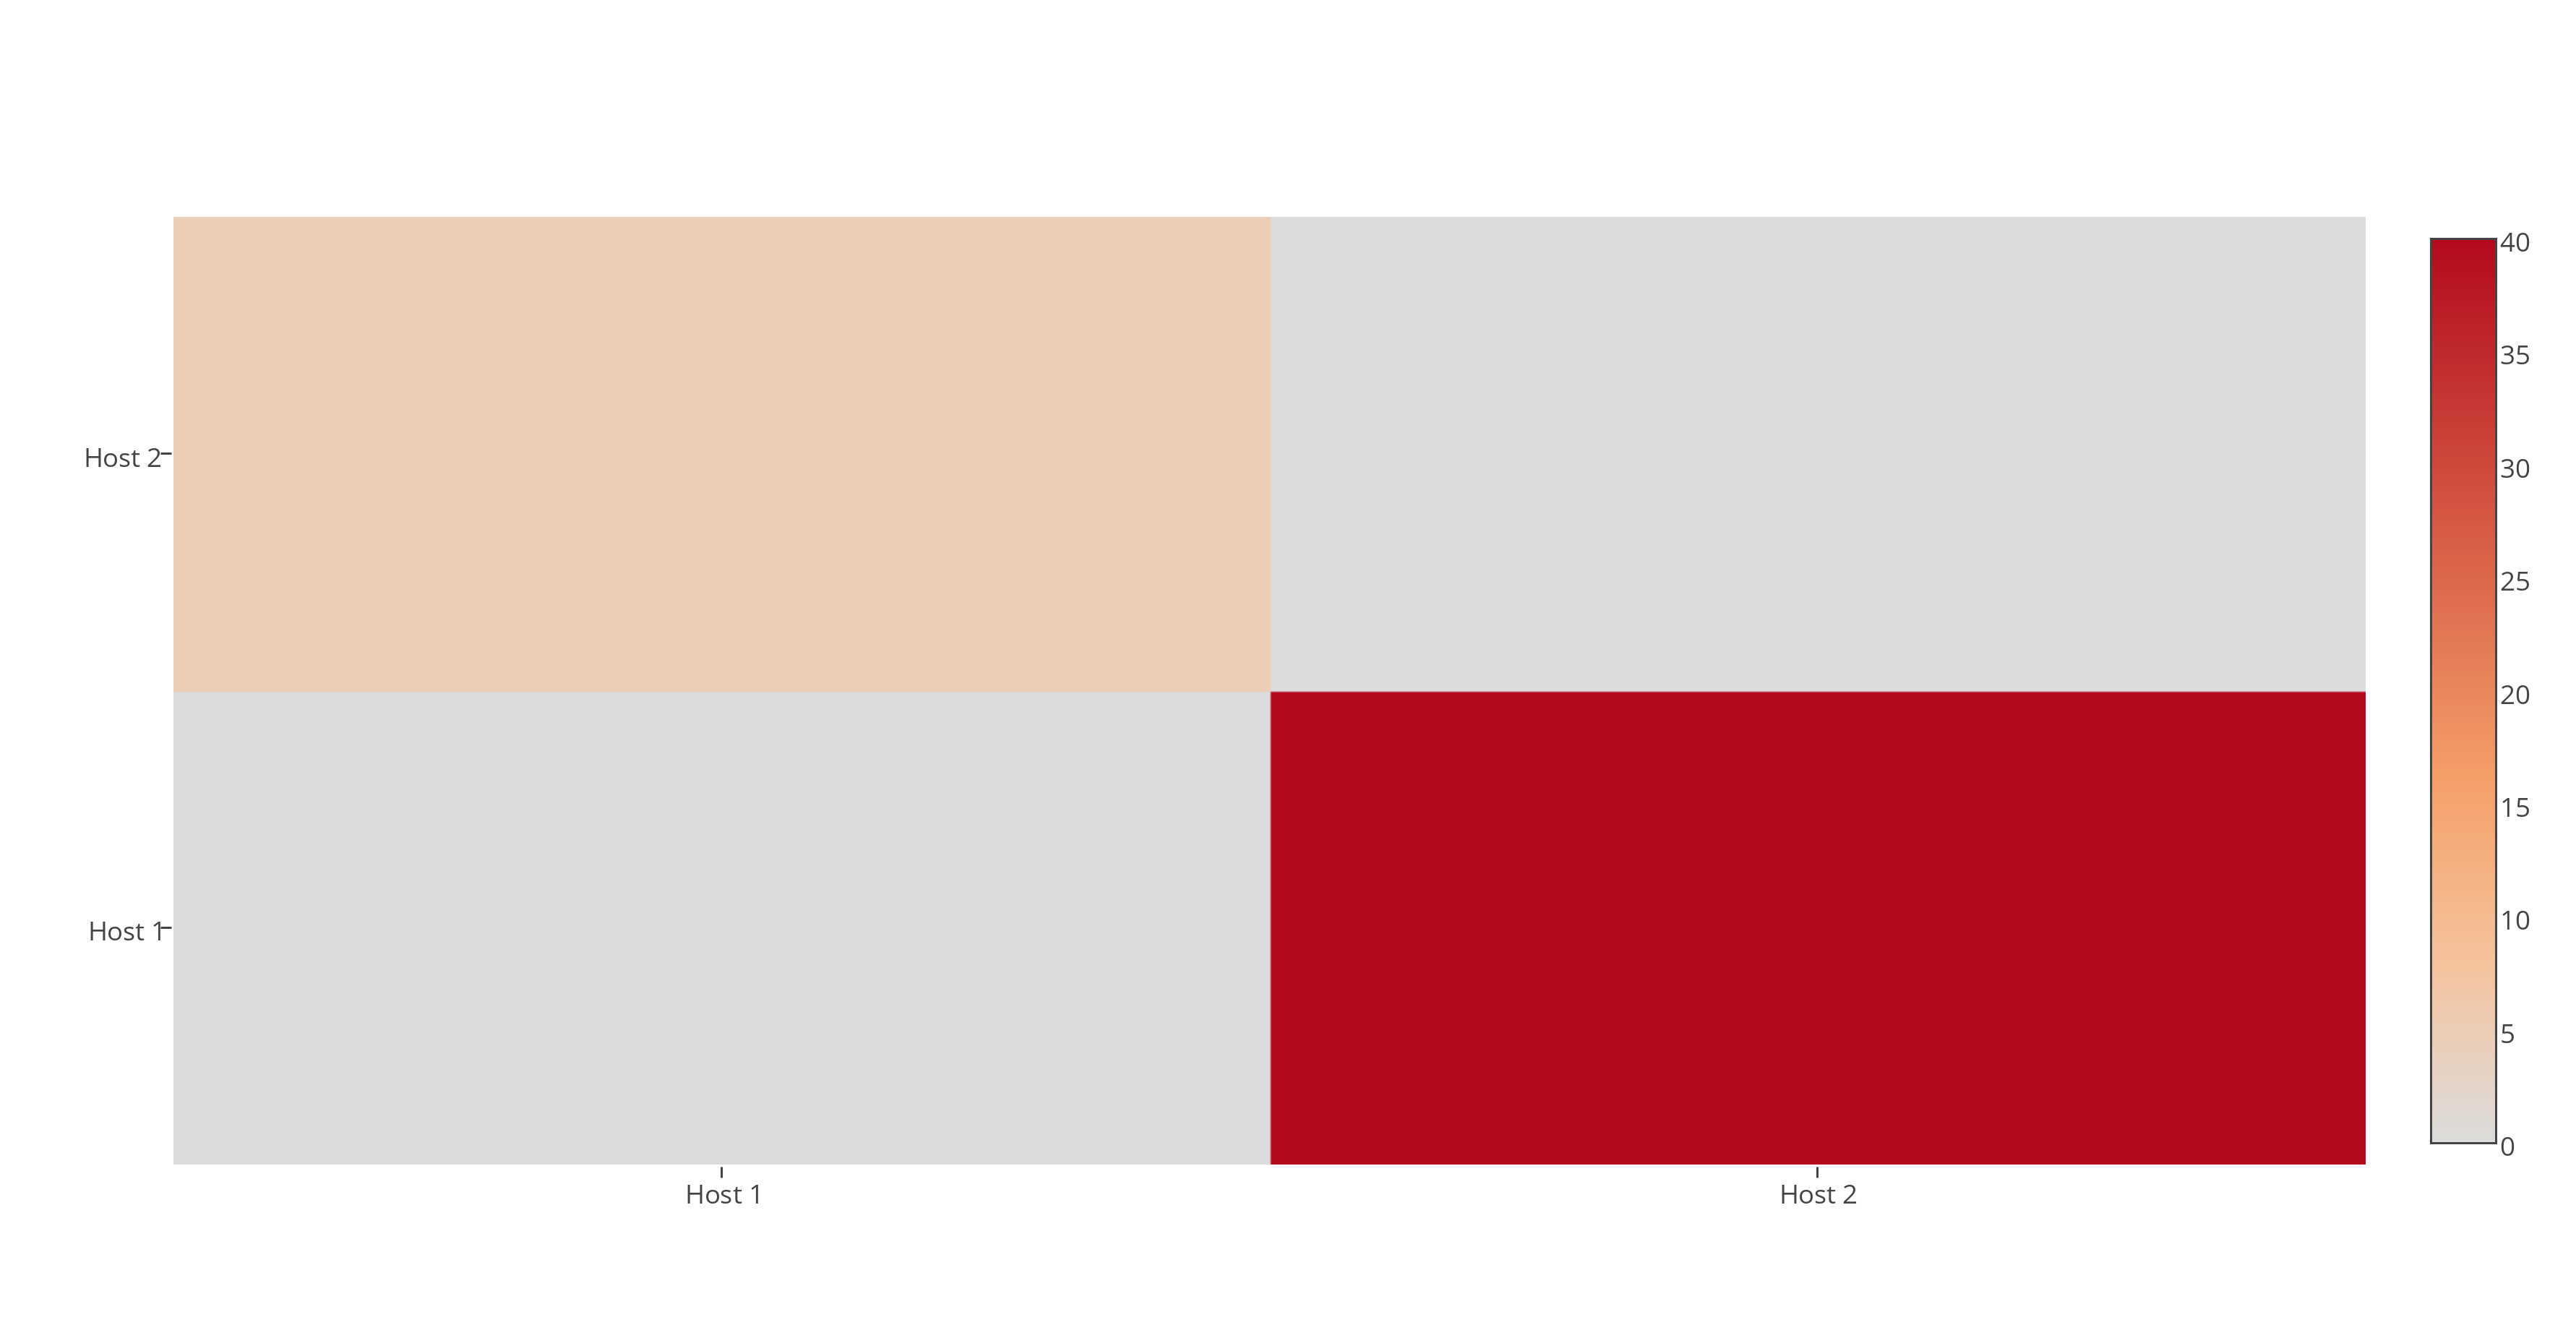
\includegraphics[width=0.9\textwidth]{host_heatmap_before}
\end{figure}

\begin{figure}[h]
\caption{Heatmap showing network traffic between different hosts after VM migration}
\centering
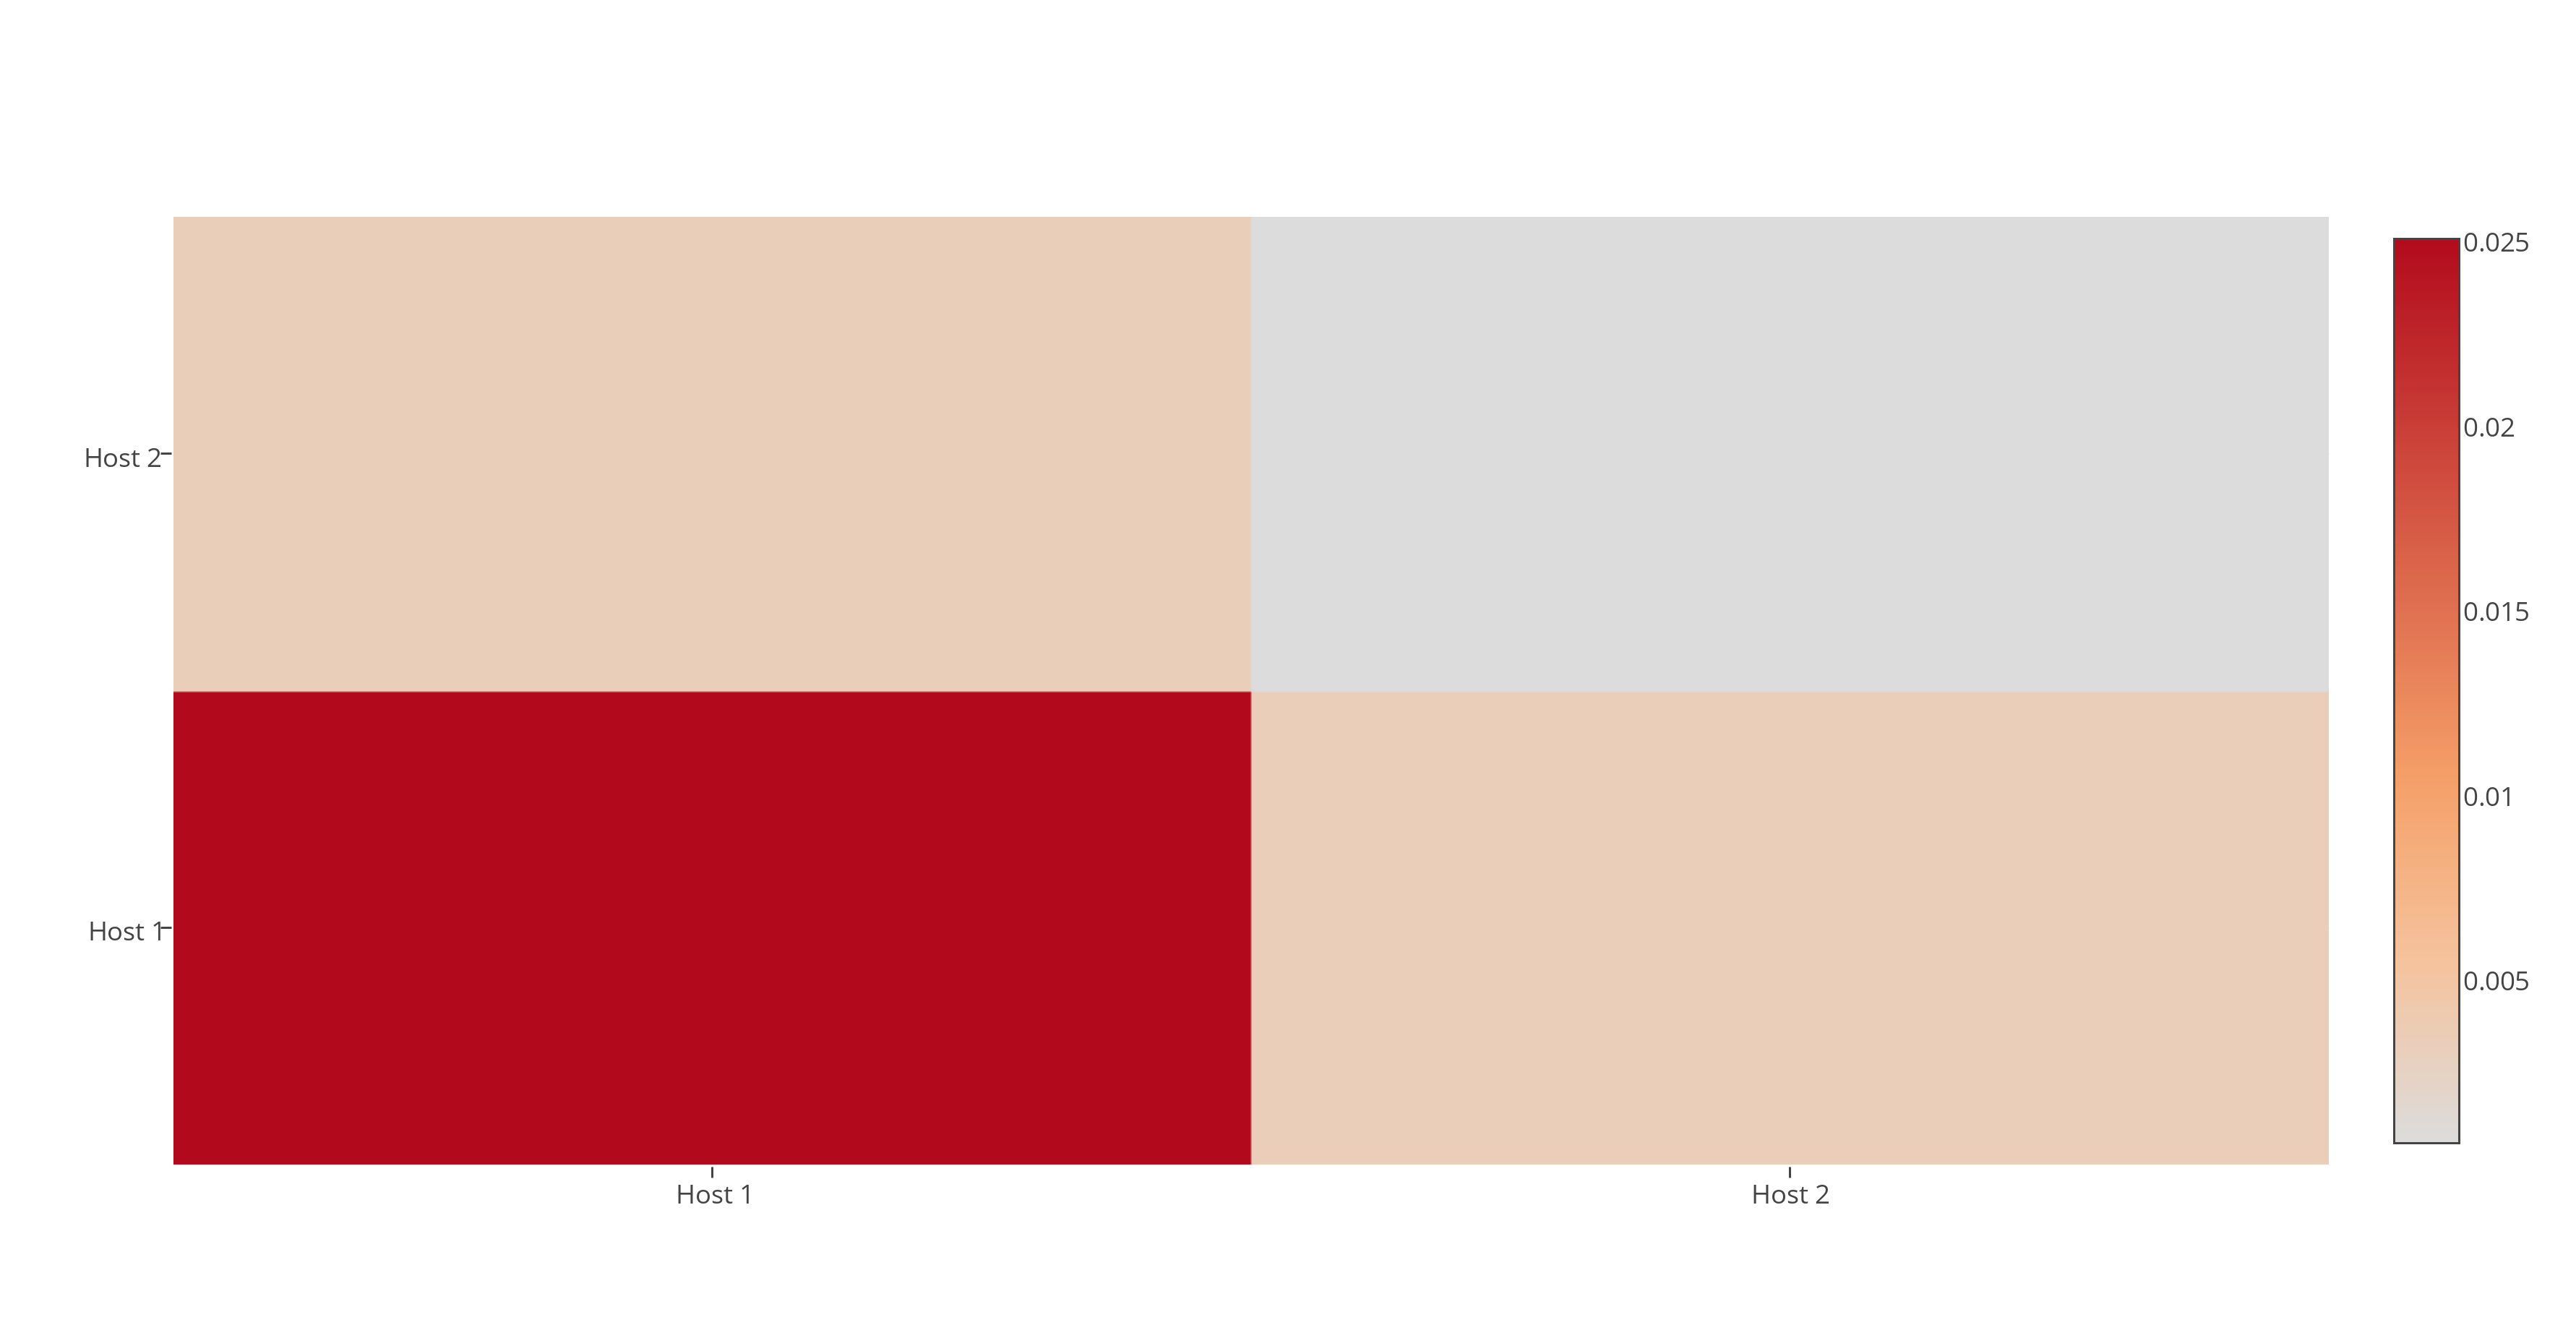
\includegraphics[width=0.9\textwidth]{host_heatmap_after}
\end{figure}

\begin{figure}[h]
\caption{Bandwidth vs time as two VMs are being consolidated on a same host}
\centering
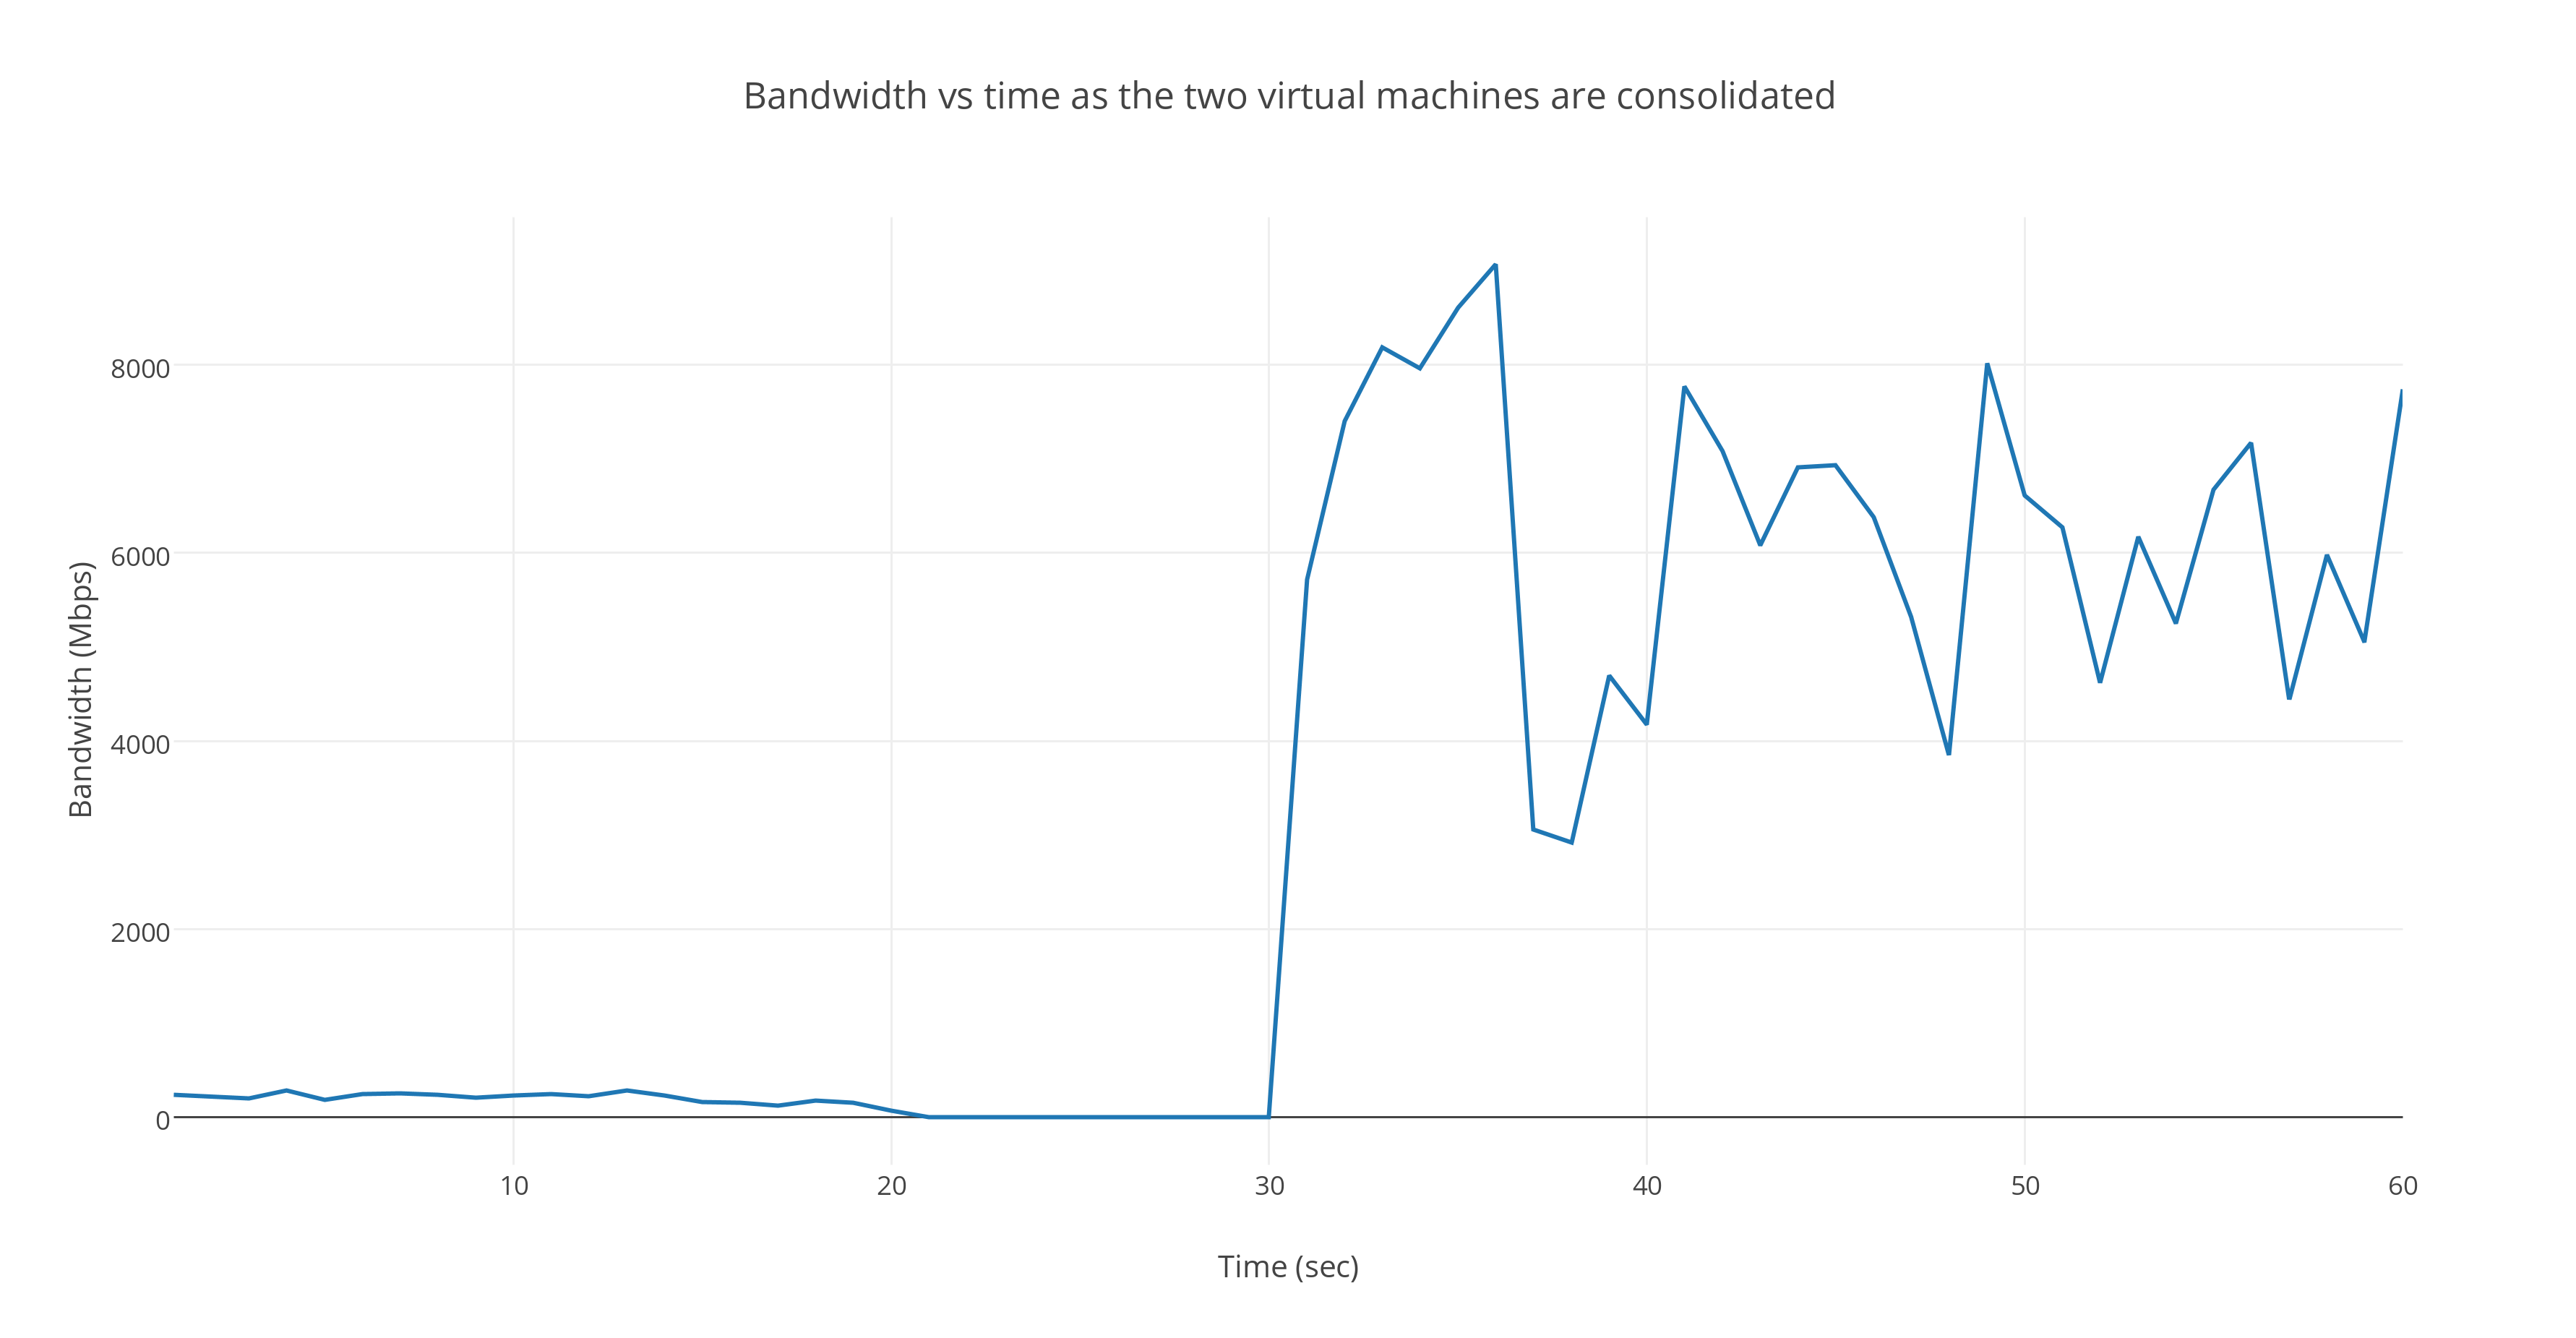
\includegraphics[width=0.9\textwidth]{bandwidth_migration}
\end{figure}

\newpage
\section{Load balancing application}
\begin{algorithm}[H]
\SetAlgoLined

\While{True}{
Read flows from the floodlight server\;
Compute the bandwidth between every pair of VMs\;
count = the number of times the bandwidth between any two VMs crosses a certain threshold in a certain time interval\;
\eIf{count exceeds pre decided number}{
find a new host for the VMs\;
start the migration\;
}{
    set the number of times the threshold has been crossed to zero\;
    continue\;
}
}
\caption{Load balancing algorithm}
\end{algorithm}

\section{Conclusion}
With the requisite understanding of the Network virtualisation and Software Defined Networking, we studied networking architecture of the baadal. We learnt about various virtual network management schemes. Based on these, we implemented some of the networking changes in the baadal. After implementing the changes, we found that there is significant improvement in the performance of the baadal in terms of bandwidth. Similarly load balancing application also brought improvemmnt in bytes transfer if two frequent talking VMs are consolidated on the same hosts. Hence we can say that SDN can be used to bring more applications in the baadal as it provides easier administratiion and control of the networking. 
\section{Future Work}
We now propose the following tasks as future work so that the SDN application can be further extended
\begin{itemize}
    \item Currently we do not handle broadcast and multicast packets in our routing scheme. These packets can be simply flooded to every output port (except the input port) if the incoming packet does not have a vlan tag. If, on the other hand, the incoming broadcast/multicast packet has a vlan tag then it can be flooded only in its vlan. The output ports corresponding to the concerned vlan can be found out using tables \textit{ipToTag}, \textit{ipToMac} and \textit{macToPort}.
    \item The connection to outside network is not established yet.It can be done by sending any packets which are destined to an outer network to the NAT machine as NAT is the only machine which is connected to the outside network. We also have to keep a track of all the fake bridges which are there for each vlan and must make sure that the packets going to outside network go through the concerned fake bridge.
    \item The load balancing module can be improved by experimenting with different vm migration algorithms.
    \item A front-end can be built which can be used to control the services that are implemented in this SDN application. Currently they are controller using the implemented REST APIs. The front-end will be able to make these REST API calls via a GUI.
\end{itemize}